\documentclass{article}

\usepackage{graphicx}
\usepackage{tikz}
\usepackage{tikzsymbols}
\usetikzlibrary{calc,patterns,shapes.geometric}
\pagestyle{empty}
\usepackage[margin=0pt]{geometry}
\geometry{papersize={14in,12in}}

\def\centerarc[#1](#2)(#3:#4:#5){\draw[#1] ($(#2)+({#5*cos(#3)},{#5*sin(#3)})$) arc (#3:#4:#5);}

\begin{document}
	\begin{figure}
		\centering
		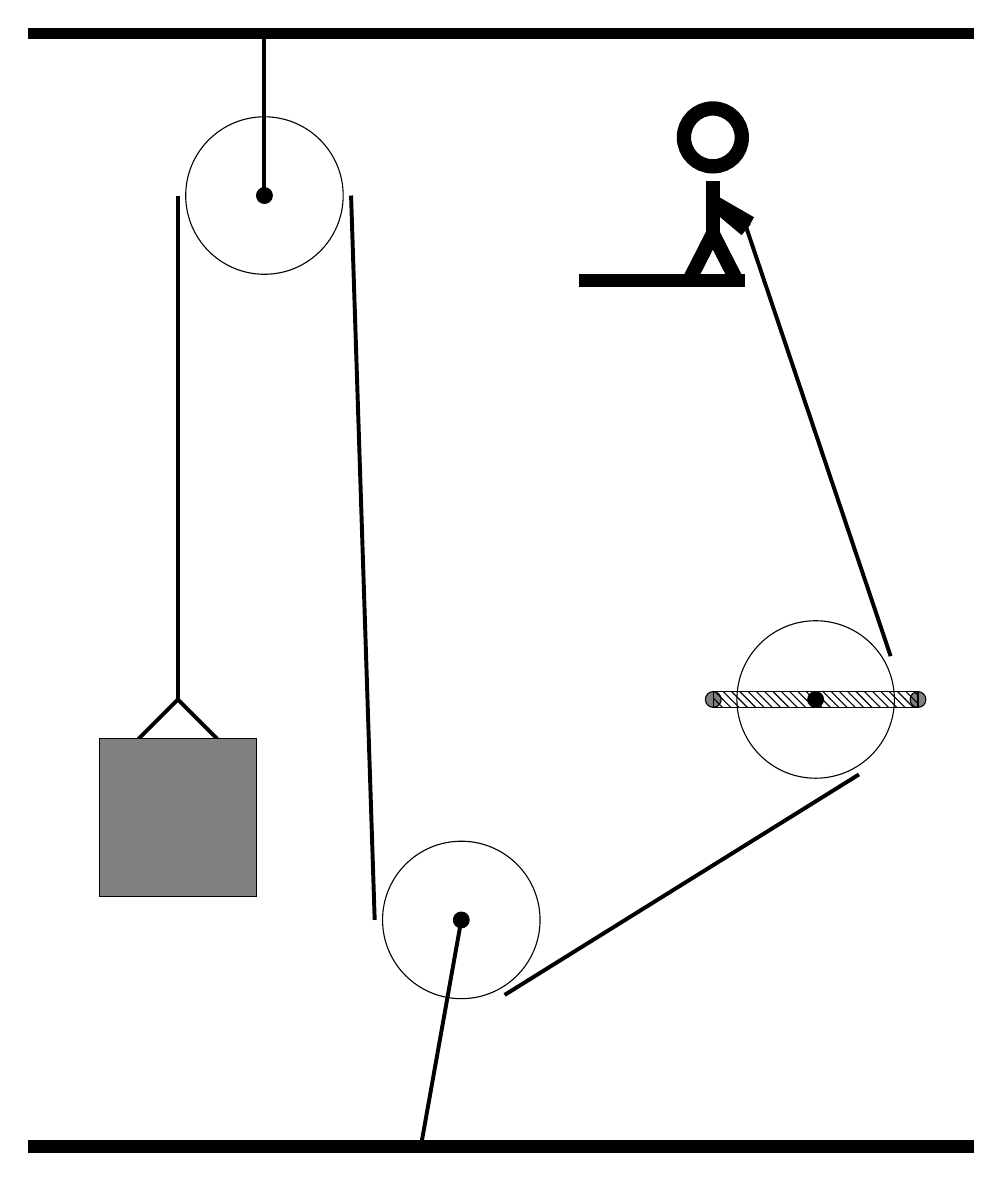
\begin{tikzpicture}
			%%%%% START %%%%%
			\draw[fill=black] (-2, 14) rectangle (10, 14.125);
			
			\draw (1, 12) circle (1);
			\draw[fill=black] (1, 12) circle (0.1);
			\draw[line width=0.5mm] (1, 14) -- (1, 12);
			
			\draw (3.5, 2.8) circle (1);
			\draw[fill=black] (3.5, 2.8) circle (0.1);
			\draw[line width=0.5mm] (3.5, 2.8) -- (3.0, 0);
			
			\draw[fill=white](8, 5.6) circle (1);
			\draw[fill=black] (8, 5.6) circle (0.1);
			\draw[fill=black!50] (9.3, 5.6) circle (0.1);
			\draw[fill=black!50] (6.7, 5.6) circle (0.1);
			\draw[pattern=north west lines, pattern color=black] (6.7, 5.7) rectangle (9.3, 5.5);
			
			\draw[line width=0.5mm](-0.6, 5.1) --  (-0.1, 5.6) -- (0.4, 5.1);
			\draw[fill=black!50] (-1.1, 5.1) rectangle (0.9, 3.1);
			
			\draw[line width=0.5mm](-0.1, 12) -- (-0.1, 5.6);
			\centerarc[line width=0.5mm](1, 12)(180:0:1.1)
			\draw[line width=0.5mm](2.1, 12) -- (2.4, 2.8);
			\centerarc[line width=0.5mm](3.5, 2.8)(180:300:1.1);
			\draw[line width=0.5mm](4.05, 1.8474) -- (8.55, 4.6474);
			\centerarc[line width=0.5mm](8, 5.6)(300:390:1.1);
			\draw[line width=0.5mm](8.9526, 6.15) -- (7.05, 11.8);
			
			\node at (6.75, 12) {\Strichmaxerl[10][-220][-30]};
			\draw[fill=black] (5, 11) rectangle (7.1, 10.85);
			
			\draw[fill=black] (-2, 0) rectangle (10, -0.15);
			%%%%% END %%%%%
		\end{tikzpicture}
	\end{figure}	
\end{document}